\chapter{Sparse Grids \textit{\&} Learning}

\section{Sparse Grids}
Sparse grids is a discretization technique that originates from numerical
partial differential equation.
Even though they can be used for diverse problems, we will build up
the exact amount of theory that is useful for our further study.

This chapter starts with a short description of the adaptive sparse grid
technique and then progresses to our application of choice: supervised learning.

\subsection{Basis functions}
\todo{Cite Sparse Grids basics.}
As our first building stone we define the \enquote{mother hat} function
\begin{equation}
  \label{eq:mother-hat}
  \varphi(x) = \max \left( 1 - \vert x \vert , 0 \right).
\end{equation}
\sidetitle{1-Dimensional Basis}
We now define a one-dimensional linear basis function for a level \(l\) and an index \(i\) by
\begin{equation}
  \label{eq:oned-basis}
  \varphi(x)_{l, i} = \varphi(2^l x - i).
\end{equation}
The basis function defined by the former equation are called the linear basis function.
\todo{Check correctness of formula!}
These basis functions assume that the function we want to approximate is zero on the boundaries.
This is why we use the similarily constructed ``modified linear basis functions'', as defined by Pflüger in~\cite{spatAdaptGrid}:
%https://tex.stackexchange.com/questions/128070/equation-how-to-create-nested-multiple-cases-in-latex-to-align-the-qualifiers
\newlength{\ldiff}
\setlength{\ldiff}{\widthof{$2^l x - i + 1$}-\widthof{$2 - 2^l x$}}
\begin{equation*}
\varphi_j (x) =
  \begin{cases}
    1 & \text {if } l = 1 \land i = 1,\\
    \begin{cases}
      2 - 2^l x & \hspace{\ldiff} \text{if } x \in [0, 2^{1-l}], \\
      0 & \hspace{\ldiff} \text{otherwise},
    \end{cases} & \text{if } l > 1 \land i = 1,\\
    \begin{cases}
      2^l x - i + 1 & \text{if } x \in [1 - 2^{1-l}, 0],\\
      0 & \text{otherwise},
    \end{cases} & \text {if } l > 1 \land i = 2^l - 1,\\
    \varphi(2^l x - i) & \text{otherwise},
  \end{cases}
\end{equation*}
that are identical to the basis functions defined by \cref{eq:oned-basis},
except on the boundaries, where they use extrapolation.

\todo{Can I use the same notation as bungartz's paper? At least reference it!}
We now define the multi-indices \(\bm{l}\), which denotes the level, and \(\bm{i}\), which indicates the index, i.e.~the position on the grid.
Arithmetical functions act on multi-indices element-wise, we use the relational operator
\begin{equation*}
  \bm{\alpha} \leq \bm{\beta} \iff \forall 1 \leq i \leq \alpha_i \leq \beta_d.
\end{equation*}
The l1- and the maximum-norm are defined as
\begin{equation*}
  \vert \bm{\alpha} \vert_1 = \sum_{1 \leq i \leq d} \alpha_i, \quad \vert \bm{\alpha} \vert_\infty = \max_{1 \leq i \leq d} \alpha_i .
\end{equation*}
We use \(\bm{1}\) and \(\bm{2}\) as a short-hand for \(1, \ldots, 1\) and
\((2, \ldots, 2)\) respectively.

\sidetitle{\(d\)-Dimensional Basis}
We can then construct the d-dimensional basis functions with the tensor product construction
\begin{equation*}
\varphi_{\bm{l}, \bm{i}} (\bm{x}) = \prod_{k=1}^d \varphi_{l_k, i_k} (x_k).
\end{equation*}

\subsection{Full \textit{\&} Sparse Grids}
Using those basis functions, we can create grids.
The treatment of sparse grids follows~\cite{bungartzSparse}.
Note, that using the index-set
\todo{Fix index set!}
\begin{equation*}
 G_l = \{(l,i) \quad | 1 \leq i_t \leq 2^{l_t} -1, i_t \text{ odd}, 1 \leq t \leq D\}
\end{equation*}
the d-dimensional basis functions span the hierachical subspaces
\begin{equation*}
  W_l = \operatorname{span}\{\phi_{l,i} \in G_l\}.
\end{equation*}
\sidetitle{Full Grid}
Using those subspaces, we can create the set of grid points \(G_n^\infty\) of the full grid for a level \(n\) and its corresponding approximation space \(V_n^\infty\)
\begin{align}
  G_n^\infty &= \bigcup_{\mathclap{\vert {\bm{l}} \vert_\infty \leq n}} G_{\bm{l}}, \\
  V_n^\infty &= \bigoplus_{\mathclap{\vert {\bm{l}} \vert_\infty \leq n}} W_{\bm{l}}.
\end{align}
The number of grid points and thus the degrees of freedom of \(V_n^\infty\) are in \( \BigO (2^{nd})\).
We can represent every function \(f(\bm{x})\) in \(V_n^\infty\) by
\begin{equation}\label{eq:coefficients-h2mix}
  f_{\bm{l}}(\bm{x}) = \sum_{(l,i) \in \bm{G_l}} \alpha_{ki} \varphi_{ki}(\bm{x}),
\end{equation}
as a sum over all grid points that is weighted by the so called hierachical coefficients \(\alpha_{ki}\).

Let \(\Omega = [0, 1]^d\) represent a \(d\)-dimensional interval. 
We now consider functions \(f \from \Omega \to \mathbb{R}\) with bounded mixed second derivatives
\sidetitle{Function Space}
\begin{equation*}
  D^{\bm{\alpha}} f = \frac{\partial^{\vert \bm{\alpha} \vert_1 } f}{\partial x^{\alpha_1}_1 \cdots \partial x^{\alpha_d}_d},
\end{equation*}
where \(\bm{\alpha}\) is a \(d\)-dimensional multi-index.
%\todo{Cite Sobolev space, adjust to otherwise used notation!}
These functions form a Soboloev space \(H_2^\text{mix}(\Omega)\) defined by
\begin{equation*}
  H_2^\text{mix}(\Omega) = \{ f \from \Omega \to \mathbb{R} : D^\alpha \in L_2(\Omega), \vert \alpha \vert_\infty \leq 2, u \rvert_{\alpha \partial = 0}\}
\end{equation*}

\sidetitle{Sparse Grid}
For this function space, sparse grids are a discretization methods that is a
reasonable trade-off between accuracy and efficiency.
By exchanging the \(l_\infty\) with the \(l_1\)-norm we get
\begin{align}
  G_n^1 &= \bigcup_{\vert {\bm{l}} \vert_1 \leq n + d - 1} G_{\bm{l}}, \nonumber \\
  V_n^1 &= \bigoplus_{\vert {\bm{l}} \vert_1 \leq n + d - 1} W_{\bm{l}} \label{eq:sparse-grid-space},
\end{align}
which correspond to the grid point set and the approximation space of sparse
grids respectively.
Df are of order \( \BigO (2^n n^{d-1})\)

\subsection{Adaptivity}
Sparse grids work best if the function adheres to our smoothness assumptions.
Functions that are not well behaving, such as functions that are not smooth in
some parts of their domain, are more difficult to handle.
\citeauthor{spatAdaptGrid} devised an adaptive technique that helps us to approximate challenging functions in~\cite{spatAdaptGrid}.
Instead of relying only on the theoretically optimal results of sparse grids for
functions in \(H^2_{\text{mix}}\), he described an optimisation process to
refine grids so that they adapt to the circumstances of the problem.
Because this optimisation process is computationally hard to calculate, a greedy
algorithm that approximates the optimal solution is used~\cite{spatAdaptGrid}.
The idea is quite simple: we create new grid points that are likely to capture
additional information, close to existing points.

An example can be seen in \cref{fig:adaptivity}.

\begin{figure}[thb]
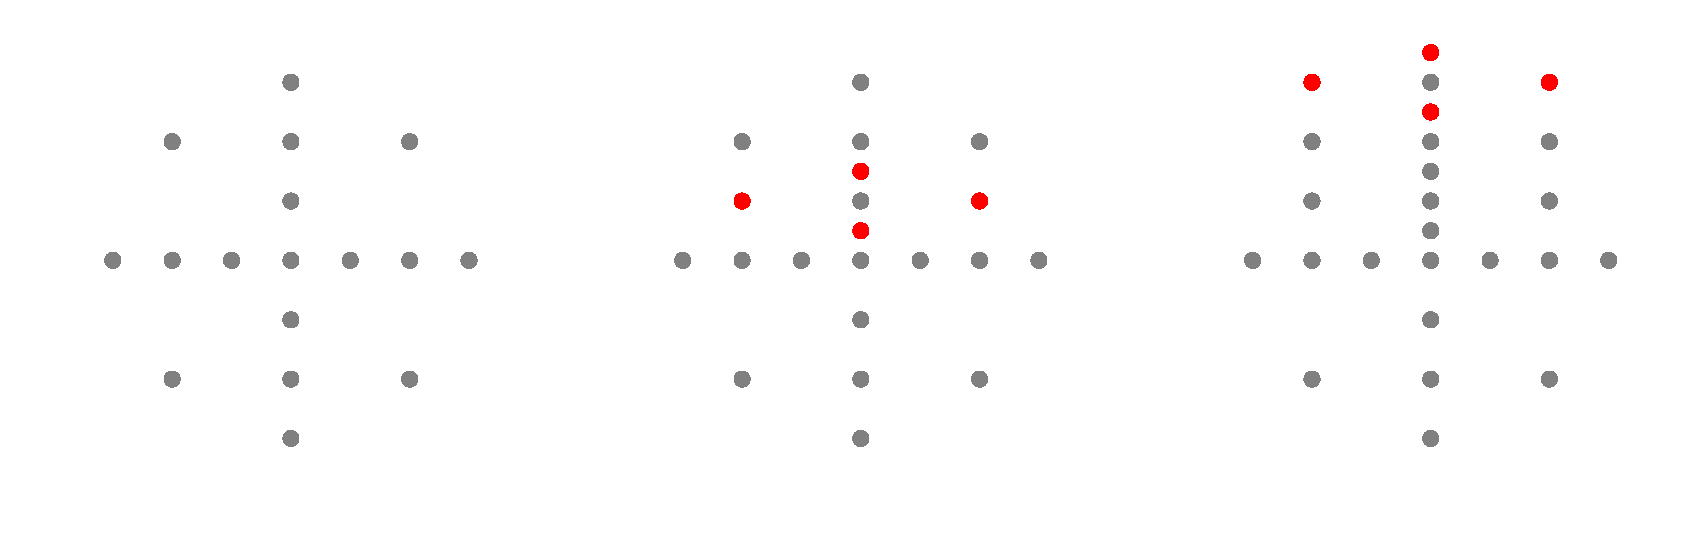
\includegraphics[width=0.7\textwidth]{adaptivity}
 \caption[Adaptivity]{We start with a small 2-dimensional grid with level 3. The first
   picture shows the standard grid, the other two show one adaptivity step each.
 The red points are the points that were created by the adaptivity step.}\label{fig:adaptivity}
\end{figure}

\section{Inference with Sparse Grids}

Let the set \todo{Fix definition for training set.}
\begin{equation*}
T = \left\{ \left(  \bm{x}, y \right) \subset \mathbb{R}^D \times y \right\} 
\end{equation*}
be a set of labelled examples with \(\bm{x}\) as predictors and \(y\) as the target variable. 
This set is called training set.
The goal is not interpolation, as we do not want to find a function that fits the examples exactly.
We rather want to find an approximation of our function that generalizes well,
that is a function that captures the structure of the training data and can be
used to predict the target variable for different, yet unseen data points.

We differentiate between
\begin{description}
\item[Regression] if we want to predict a continuous \(y\) and
\item[classification] if we want to predict a discrete value, a class.
\end{description}
In this thesis we will mostly see examples of regression, the last chapter
contains an example for a high-dimensional classification problem.

Sparse grids can be used to perform regression.
Using the matrices
\begin{equation*}
\boldsymbol{\phi}(\boldsymbol{x}) = \begin{pmatrix}
  \varphi_1(\bm{x}) \\
  \vdots \\
  \varphi_m(\bm{x})
\end{pmatrix}
, \quad
\boldsymbol{\Phi}(\boldsymbol{x}) = \begin{bmatrix}
  \boldsymbol{\phi}(x_1)^\intercal\\
  \vdots \\
  \boldsymbol{\phi}(x_n)^\intercal
\end{bmatrix},
\end{equation*}
we can express our function as
\begin{equation*}
\hat{y} = \sum_{j = 1}^m \alpha_j \varphi_{j}(\bm{x}) = \boldsymbol{\alpha}^\intercal \bm{\phi} (\bm{x}),
\end{equation*}
which is a weighted sum of the basis functions, closely related to \cref{eq:coefficients-h2mix}.

The optimisation goal is then given by
\begin{equation}\label{eq:optGoal}
\min_{\bm{\alpha}} \left\Vert  \bm{\Phi} \bm{\alpha} - \bm{y}   \right\Vert_2^2  + \lambda \mathcal{S}(\bm{\alpha}), 
\end{equation}
where \(\mathcal{S}(\bm{\alpha})\) is a regularization operator and \(\lambda\) is a constant.
This least-square problem can be solved for differentiable operators
\(\mathcal{S}\) by a conjugated-gradient-solver.
Adaptivity can be integrated into this process by performing a refinement step
after solving the optimisation step, iterating until a satisfactory performance
is archived.
We perform adaptivity by calculating \textsc{MSE} for the model and then refine
the grid, starting with the point with the highest contribution to the error.

A binary classification problem can be transformed into a regression problem,
by relaxing the target \(y\).
We set \(y = 0\) for each dataset when the datum belongs to the first class, and
\(y = 1\) if it does not.
The prediction of the model can then be interpreted as a certainty that the
data is a member of the class.

To solve a multi-class-classification problem, one-vs-all classification is used,
for which we transform the problem into multiple binary classification problems.
To perform a prediction we calculate the results for each binary estimator, and
report the class label of the learner that returned the largest certainty.

This implies that all methods that improve the performance of the regression procedure also very likely lead to better classification results, because we are performing classification via regression.
%%% Local Variables:
%%% mode: latex
%%% TeX-master: "../main"
%%% End: